\documentclass[a4paper,11pt,twoside]{report}
\usepackage[T1]{fontenc}
\usepackage[frenchb]{babel} %active le mode français
\usepackage[latin1,utf8]{inputenc} % Mettre des accents
\usepackage[top=2cm , bottom=2cm , left=2cm , right=2cm]{geometry} %propriétés de notre page
\usepackage{amsmath} %liste de symboles et applications mathématiques
\usepackage{amsfonts} %idem
\usepackage{color} %Permet d'utiliser la couleur dans nos documents
\usepackage[usenames,dvipsnames]{xcolor}
\usepackage{listings} %Paquet de coloration syntaxique (langages)
\usepackage{hyperref} % Créer des liens et des signets 
\usepackage[babel=true]{csquotes} %permet les quotations (guillemets)
\usepackage{graphicx} %Importation d'image
\usepackage{fancyhdr} %en-tête et pieds de page+
\usepackage{lastpage} %permet d'obtenir le nombre total de page
\usepackage{multido}
\usepackage{eurosym}
\usepackage{listingsutf8}
\usepackage{tikz}
\usepackage{ulem}
\usepackage{colortbl} %permet de mettre de personnaliser les colones des tabular
\usepackage{pdfpages}
\usepackage{appendix} %annexes
\setlength{\headheight}{15pt}
\lstset{language=C,
	breaklines=true,
	numbers=left,
	keywordstyle=\color{blue},
	commentstyle=\color{Gray},
	stringstyle=\color{red},
	tabsize=4,
	framexleftmargin=7mm,
	frame=single
	}
% Informations du rapport
\title {Rapport de TP \\ Problème de production de type ULS}
\author {Quentin Tonneau - Camille Drancourt}
\date{}
\renewcommand{\thesection}{\arabic{section}}
%Propriétés des liens
\hypersetup{
colorlinks=true, %colorise les liens  
urlcolor= blue, %couleur des hyperliens 
linkcolor= blue,%couleur des liens internes
citecolor=black
} 
%\setlength{\parindent}{0cm}
\addto\captionsfrench{
	\renewcommand{\chaptername}{Partie}
}

\fancypagestyle{plain}
{

	\fancyhead{}
	\fancyfoot{}
	\lhead{Quentin Tonneau - Camille Drancourt}
	\rhead{Université de Nantes}
	\chead{Problème de production de type ULS}
}
\begin{document}
\tableofcontents
\newpage

\chapter{Description du problème}
Le problème de planification de production étudié dans cet exercice est appelé \textit{Uncapacitated Lot-Sizing Problem}. Comme son nom l'indique, il n'y a dans ce cas précis aucune contrainte de capacité ou de limite de production.
Le plan de production est décomposé en T instances, dont on cherche à décider l'ouverture ou non ($y_t$), ainsi que la quantité d'éléments à produire $x_t$. L'ouverture d'une instance entraîne un coût fixe ($f_t$), ainsi qu'un coût unitaire de production ($p_t$).
Il faut impérativement subvenir aux demandes des clients pour tout instant $t$, mais il est possible à une instance $t$ de produire plus que nécessaire, et stocker l'ensemble de la ``surproduction'' ($s_t$) jusqu'à $t+1$ moyennant un coût unitaire de $h_t$.


Nous tentons dans cette analyse de résoudre quelques instances de ce problème via un algorithme de \textbf{branch \& bound}, et nous essayons de comprendre quelles sont les astuces de modélisation et les choix de résolution permettant d'améliorer au fur et à mesure notre rapidité de résolution.

\chapter{Le projet initial}
\section{La modélisation}
Les algorithmes de branch \& bound sont très utiles pour résoudre des problèmes en variables entières, en effectuant une série de résolution du problème ``relaché'' et en introduisant à chaque étape une nouvelle contrainte d'intégrité sur une des variables de décision.
Nous introduisons donc un modèle correspondant au problème ci-dessus, mais dont les variables entières ou binaires ($y_t$) ne possèdent pas de contraintes d’intégrité.

Voici le modèle proposé :
\[
 \left[ \begin{matrix}
         min z= & \displaystyle \sum_{t\in \{1...T\}} y_t \times f_t + x_t \times p_t + s_t \times h_t \\
         s/c & s_{t-1}+x_{t}& =d_t+s_t & \forall t\in \{0...T\} \\
         & y_t*M &\geq x_t \\
         &s_0&=0\\
         &s_t&=0\\
         &y_t,x_t,s_t&\geq 0
        \end{matrix}
 \right]
\]
La première contrainte, que nous appelons contrainte d'équilibre, impose l'absence de perte de produit lors de la production. En effet, l'ensemble des éléments entrants (stock précédent et production) soit être égal à l'ensemble des éléments sortants (ventes et stock).
La seconde contrainte implémente une constante M très grande imposant l'ouverture de l'instance si au moins un élément est produit par cette instance.
Les contraintes (3) et (4) indiquent l'état du stock au départ et à l'arrivé, fixés ici à 0.

\section{L'algorithme}
Pour résoudre entièrement le problème, nous avons exécuté à la main l'algorithme du branch \& bound en effectuant les choix suivants :
\begin{itemize}
 \item Relâcher ou contraindre les variables $y_t$ à 0 ou 1.
 \item Toujours choisir la variable $y_t$ la plus proche de 0 et la fixer à 0 (dans un premier temps)
\end{itemize}

\section{L'implémentation}
Nous utilisons pour la résolution le solveur GLPK sous sa forme ``lpsolve''. L'implémentation de la modélisation dans ce langage est donné en Annexe \ref{implementationlpsolve}
Afin de contraindre une variable, nous ajoutons à chaque étape une ligne de type :
\begin{verbatim}
 s.t. contrX :y[A]=B;
\end{verbatim}
 avec A=$t$ et B$\in \{0,1\}$
 
 Nous fixons également M à 100, valeur arbitrairement grande.
\section{Résultats}
L'exécution de l'algorithme de branch\&bound nous permet d'obtenir l'arbre de la figure \ref{graph1}
\begin{figure}[h]
 \centering
 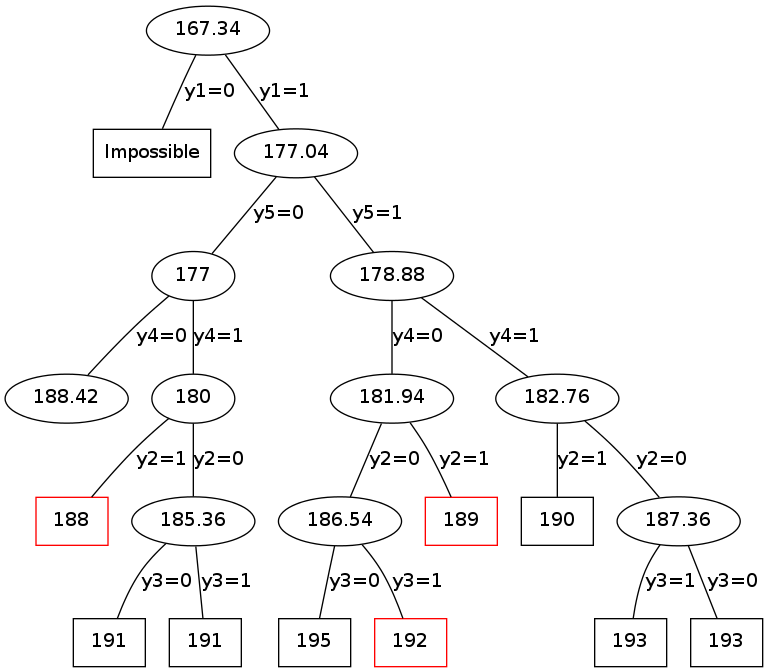
\includegraphics[width=0.8\textwidth]{graph1.png}
 \caption{Arbre initial}
 \label{graph1}
\end{figure}

On obtient un résultat optimal égal à 188, avec de très nombreuses branches et n\oe{}uds parcourus. Les choix de variables et de valeurs (algorithme de branch\&bound) ne sont pas optimaux, et il est sûrement possible d'améliorer notre modélisation ou notre système de résolution.
\chapter{Amélioration du modèle}
\section{Les valeurs des variables}
Le seul élément variable dans notre modélisation est $M$. En cherchant à améliorer la précision des résolution du problème relâché dans notre branch\&bound, nous arrivons à la conclusion suivante :

Plus M est petit, plus l'encadrement des valeurs possibles de chaque $y_t$ est petite. La valeur retournée par le solveur est donc plus proche de la valeurs maximum réelle.
Il faut cependant toujours conserver un M supérieur à la production maximale de chaque instance. On remarque, que la production maximale d'une instance est égale à la demande totale des clients. En effet, nous pourrions choisir de produire tous les éléments lors de la première instance, puis de répartir la production sur toutes les instances suivantes.
Dans l'instance donnée, $M$ doit être supérieure ou égale à 25. En modifiant M à 25, nous obtenons un arbre très similaire à la première résolution.

Afin d'améliorer encore notre modélisation, nous observons que la valeur maximale de M dépend de l'instance $t$. En effet, on ne peut produire au maximum que la demande totale \textbf{restante}.
Dans l'instance donnée, M devient donc un tableau de $5$ valeurs égales à $\{25, 22, 17, 11, 8\}$. Nous reprenons alors l'algorithme de branch\&bound, et nous obtenons l'arbre de la figure \ref{graph2}\\
\begin{figure}[h]
 \centering
 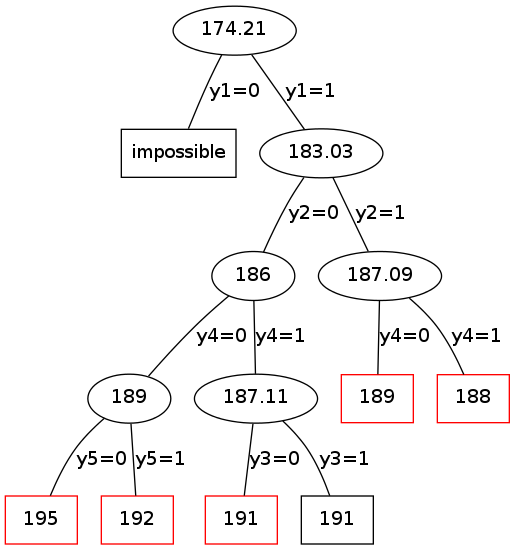
\includegraphics[width=\textwidth/2]{graph2.png}
 \caption{Modification de la valeur de M : tableau}
 \label{graph2}
\end{figure}



\section{Contraintes de coupes et inégalités valides}



\section{Étude de la structure des solutions}



\section{Cas Wagner-Whitin}
Nous sommes dans un cas de coûts de Warner-Within lorsqu'il est systématiquement plus coûteux de produire et de stocker un produit pour une instance ultérieure, que de produire directement à l'instance $t$ (unitairement).
Un exemple de cas est donné dans le tableau \ref{warner1}
\begin{table}[h]
  \centering
 \begin{tabular}{|c|ccccc|}
\hline
$t$&1&2&3&4&5\\\hline\hline
$d_t$&3&5&6&3&8\\
$p_t$&3&4&4&8&3\\
$h_t$&2&1&5&1&-\\
$f_t$&10&8&6&4&2\\\hline
\end{tabular}
 \caption{Exemple de cas : Warner-Within}
 \label{warner1}
\end{table}

La logique nous amène alors à une résolution simple : On ne stocke jamais de produit, et on produit pour chaque instance $t$ la demande $d_t$ associée. Néanmoins, nous ne pouvons pas appliquer cette méthode directement.
En effet, si le gain total obtenu ($(p_t-s_{t-1})\times d_t$) est inférieur au coût initial de l'instance $t$ ($f_t$), alors il est plus intéressant de stocker. 

\section{Instance finale}


\chapter{Conclusion}








\begin{appendices}
\chapter{Implémentation lpsolve}
\label{implementationlpsolve}
\begin{verbatim}
 #Données
param nbpostes;

set T:=1..nbpostes;
set T2:=0..nbpostes;
param M:=100;

param d{T};
param h{T};
param p{T};
param f{T};

#Variables de décision
var x{T} >=0;
var y{T} >=0;
var s{T2}>=0;

#Fonction objectif
minimize couts : sum{i in T} (y[i]*f[i] + x[i]*p[i] + h[i]*s[i]);

#Contraintes

s.t. Equilibre{i in T} : (s[i-1]+x[i])=(s[i]+d[i]);
s.t. Activation{i in T}: y[i]*M >= x[i];
s.t. contr1 :s[0]=0;
s.t. contr2 :s[nbpostes]=0;

#Résolution
solve;

#Affichange des res
display : s;
display : x;
display : y;
display : sum{i in T} (y[i]*f[i] + x[i]*p[i] + h[i]*s[i]); #fonction objectif à recopier

data;

param nbpostes:= 5;
param d:= 1 3 2 5 3 6 4 3 5 8;
param p:= 1 2 2 4 3 6 4 8 5 10 ;
param h:= 1 3 2 2 3 3 4 2 5 0;
param f:= 1 10 2 8 3 6 4 4 5 2;

end;
\end{verbatim}
\end{appendices}

\end{document}

